\begin{exercise}
\begin{figure}[H]
\centering
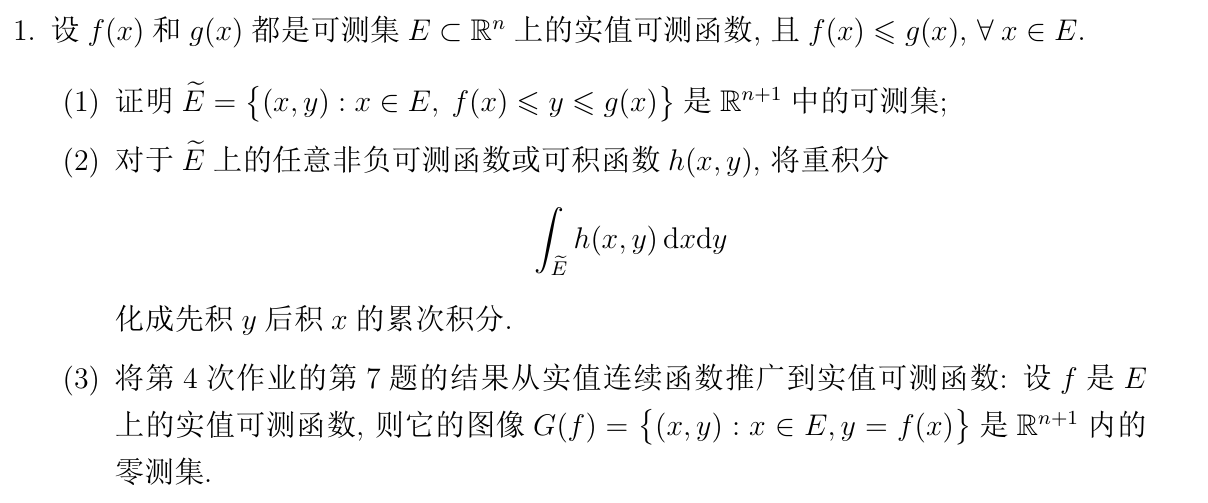
\includegraphics[width=\textwidth]{hw15-2025061015.png}
% \caption{}
\label{}
\end{figure}
\end{exercise}
\begin{proof}
证明思路:

\begin{enumerate}
	\item 我们定义两个辅助函数 $\phi(x, y)=y-f(x)$ 和 $\psi(x, y)=g(x)-y$。
	\item 由于 $f(x)$ 和 $g(x)$ 是 $E$ 上的可测函数,我们可以将它们延拓到整个 $\mathbb{R}^n$ 上(例如,在 $E^c$ 上令它们为 0 或 $\infty$ ),这样它们就成为 $\mathbb{R}^n$ 上的可测函数。函数 $y$ 作为变量 $y$ 的函数是连续的,因此也是可测的。
	\item 可测函数的和、差仍然是可测函数。因此,$\phi(x, y)$ 和 $\psi(x, y)$ 是在 $\mathbb{R}^{n+1}$ 上的可测函数。
	\item 根据可测函数的定义,对于任意实数 $a$ ,集合 $\{(x, y): \phi(x, y)>a\}$ 是可测集。我们取 $a=$ 0 ,则集合 $A=\{(x, y): y-f(x) \geq 0\}=\{(x, y): f(x) \leq y\}$ 是 $\mathbb{R}^{n+1}$ 中的可测集。
	\item 同理,集合 $B=\{(x, y): g(x)-y \geq 0\}=\{(x, y): y \leq g(x)\}$ 也是 $\mathbb{R}^{n+1}$ 中的可测集。
	\item 集合 $E \times \mathbb{R}$ 在 $\mathbb{R}^{n+1}$ 中是可测的,因为 $E$ 是 $\mathbb{R}^n$ 中的可测集。
	\item 集合 $\tilde{E}$ 可以表示为这三个可测集的交集:
\end{enumerate}
\[
	\tilde{E}=\{(x, y): x \in E, f(x) \leq y \leq g(x)\}=(E \times \mathbb{R}) \cap A \cap B
\]
\begin{enumerate}
	\item 有限个可测集的交集仍然是可测集。因此,$\tilde{E}$ 是 $\mathbb{R}^{n+1}$ 中的可测集。
\end{enumerate}

\end{proof}
\begin{proof}
利用 Fubini-Tonelli 定理:
\[
\int_{\widetilde{E}}^{} h(x,y) \, \mathrm{d}x \mathrm{d}y=\int_{E}^{} \int_{f(x)}^{g(x)} h(x,y) \, \mathrm{d}y  \, \mathrm{d}x
\]
\end{proof}

\begin{proof}
\[
G(f)=\{ (x,y):x\in E ,f(x)\leq y\leq f(x)\}
\]
于是
\[
m_{n+1}(G(f))=\int_{G(f)}^{} 1 \, \mathrm{d}x \mathrm{d}y=\int_{E}^{} \underbrace{ \int_{f(x)}^{f(x)} 1 \, \mathrm{d}y }_{ =0 }  \, \mathrm{d}x=0 
\]
\end{proof}

\begin{exercise}
\begin{figure}[H]
\centering
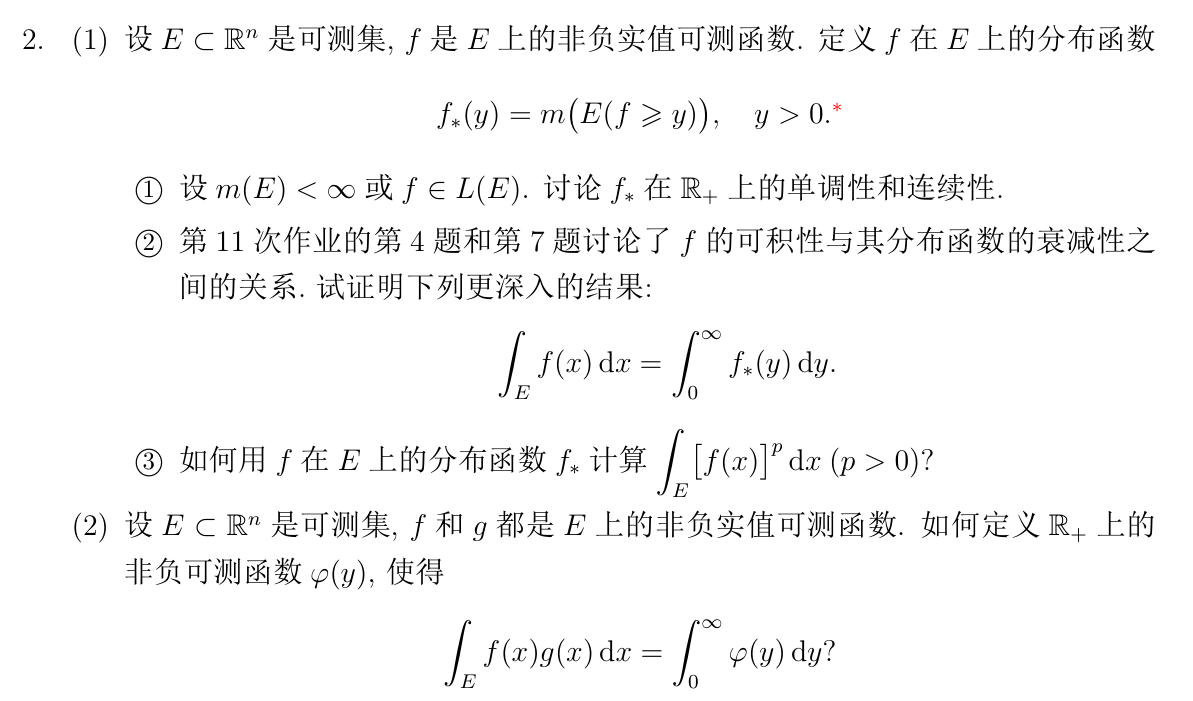
\includegraphics[width=\textwidth]{1-hw15-2025061015.png}
% \caption{}
\label{}
\end{figure}
\end{exercise}
(1)
$f_{*}(y)$ 单调不增. 因为 $0<y_1<y_2\Rightarrow E(f\geq y_2)\subseteq E(f\geq y_1)$.

$f_{*}(y)$ 在 $(0,+\infty)$ 上左连续. 给定 $y_0>0$,任取 $\{ y_k \}_{k\geq1}$ 递增趋于 $y_0$,$A_k=E(f\geq y_k)$. 那么 $A_1\supseteq A_2\supseteq\dots$. 交集 $\cap_{k\geq1}A_k=E(f\geq y_0)$. 若有 $m(A_1)<\infty$,那么
\[
\lim_{ k \to \infty } m(A_k)=m(\cap_{k\geq 1}A_k)=m(E(f\geq y_0))=f_{*}(y_0)
\]
根据连续极限的定义,$\lim_{ y \to y_0^{-} }f_{*}(y_0)=f_{*}(y_0)$.

接下来说明:若 $m(E)<\infty$,则 $m(A_1)\leq m(E)<\infty$;若 $f$ 可积,则 $m(A_1)=\int_{E(f\geq y_1)}^{} 1 \, \mathrm{d}x\leq\frac{1}{y_1}\int_{E(f\geq y_1)}^{} f(x) \, \mathrm{d}x\leq\frac{1}{y_1}\int_{E}^{} f(x) \, \mathrm{d}x<\infty$.

由 Tonelli 定理:
\[
\int_{0}^{\infty} f_{*}(y) \, \mathrm{d}y =\int_{0}^{\infty} \int_{E}^{} \chi_{E(f\geq y)} \, \mathrm{d}x  \, \mathrm{d}y=\int_{E}^{} \int_{0}^{f(x)} 1 \, \mathrm{d}y \, \mathrm{d}x =\int_{E}^{} f(x) \, \mathrm{d}x
\]
\[
\begin{aligned}
\int_{0}^{\infty} [f(x)]^{p} \, \mathrm{d}x  & =\int_{0}^{\infty} \int_{E}^{} \chi_{E(f^{p}\geq  y)} \, \mathrm{d}y  \, \mathrm{d}x  \\
 & =\int_{0}^{\infty} \int_{E}^{}\chi_{E\left( f\geq y^{\frac{1}{p}} \right)}  \, \mathrm{d}y  \, \mathrm{d}x  \\
 & =\int_{0}^{\infty} f_{*}\left( y^{\frac{1}{p}} \right) \, \mathrm{d}y \\
 & \overset{ t=y^{\frac{1}{p}} }{ = }p\int_{0}^{\infty} t^{p-1}f(t) \, \mathrm{d}t 
\end{aligned}
\]
(2)
由于 $f,g$ 在 $E$ 上非负可测,那么 $fg$ 也非负可测. 这个证明可以利用简单函数逼近,比如
\[
0\leq \varphi_1\leq \varphi_2\leq \dots\to f(x)
\]
\[
0\leq \psi_1\leq \psi_2\leq \dots\to g(x)
\]
于是 $h_n\coloneqq\varphi _n\psi _n$ 也是简单函数,
\[
0\leq h_1\leq h_2\leq \dots\to f(x)g(x)
\]
于是 $fg$ 可测.

或者利用分解 $fg=\frac{1}{4}[(f+g)^{2}-(f-g)^{2}]$.

\begin{itemize}
	\item 定理 1:若 $f_1, f_2$ 是可测函数,则它们的和 $f_1+f_2$ 与差 $f_1-f_2$ 也是可测函数。
	\item 定理 2:若 $f$ 是可测函数,$c$ 是常数,则 $c f$ 也是可测函数。
	\item 定理 3:若 $f$ 是可测函数,$\phi$ 是一个连续函数(更一般地,是 Borel 可测函数),则复合函数 $\phi \circ f$ 也是可测函数。特别地,如果 $f$ 可测,那么 $f^2$ 也是可测的,因为可以令 $\phi(t)=t^2$ ,这是一个连续函数。
\end{itemize}

故 $fg$ 可测.

我们定义 $\varphi(y)$ 如下:
\[
\varphi(y)=m(\{x \in E: f(x) g(x) \geq y\}), \quad y>0
\]
这个函数 $\varphi(y)$ 是非负的并且是可测的(因为它是一个单调函数)。根据上述推理,这个定义满足给定的等式:
\[
\int_E f(x) g(x) d x=\int_0^{\infty} \varphi(y) d y
\]
\begin{exercise}
\begin{figure}[H]
\centering
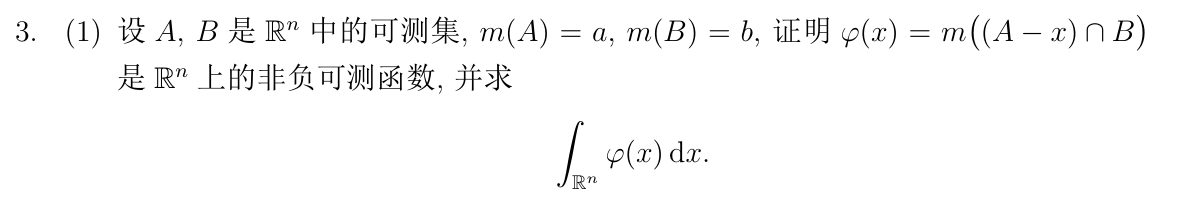
\includegraphics[width=\textwidth]{2-hw15-2025061015.png}
% \caption{}
\label{}
\end{figure}
\begin{figure}[H]
\centering
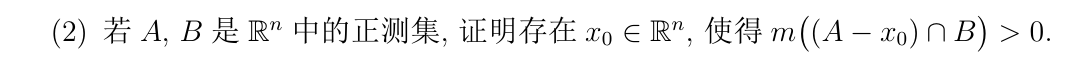
\includegraphics[width=\textwidth]{3-hw15-2025061015.png}
% \caption{}
\label{}
\end{figure}
\end{exercise}
(1)
\[
\begin{aligned}
\int_{\mathbb{R}^{n}}^{} \varphi(x) \, \mathrm{d}x  & =\int_{\mathbb{R}^{n}}^{} \int_{\mathbb{R}^{n}}^{} \chi_{A-x}\cdot \chi_{B} \, \mathrm{d}y  \, \mathrm{d}x   \\
 & =\int_{\mathbb{R}^{n}}^{} \int_{\mathbb{R}^{n}}^{} \chi_{x+y\in A}\cdot \chi_{y \in B} \, \mathrm{d}y  \, \mathrm{d}x  \\
 & =\int_{\mathbb{R}^{n}}^{} \int_{\mathbb{R}^{n}}^{} \chi_{z\in A}\cdot \chi _{y\in B} \, \mathrm{d}y \, \mathrm{d}z \\
  & =ab
\end{aligned}
\]
(2)
若对于任意 $x\in \mathbb{R}^{n}$,都有 $m((A-x)\cap B)=0$. 那么
\[
0<ab=\int_{\mathbb{R}^{n}}^{} \varphi(x) \, \mathrm{d}x =\int_{\mathbb{R}^{n}}^{} 0 \, \mathrm{d}x =0
\]
矛盾!

\begin{exercise}
\begin{figure}[H]
\centering
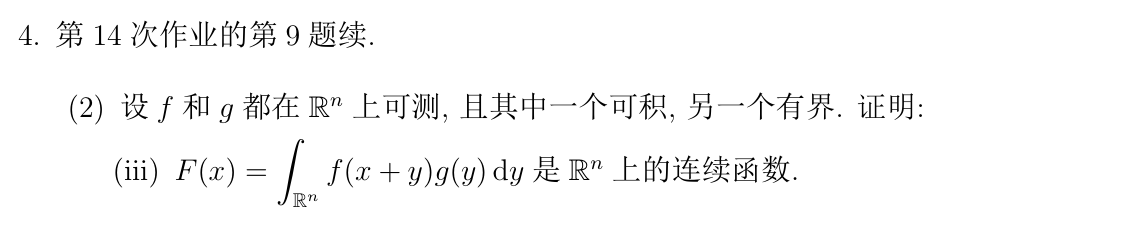
\includegraphics[width=\textwidth]{4-hw15-2025061015.png}
% \caption{}
\label{}
\end{figure}
\end{exercise}
不妨设 $g$ 有界,$f$ 可积,那么
\[
\lvert F(x) \rvert \leq \int_{\mathbb{R}^{n}}^{} \lvert f(x+y)g(y) \rvert  \, \mathrm{d}y \leq M\cdot\lVert f \rVert _{L^{1}(\mathbb{R}^{n})}<\infty
\]
故 $F$ 良好定义.

对于 $h>0$,考虑
\[
\begin{aligned}
\lvert F(x+h)-F(x) \rvert  & \leq \int_{\mathbb{R}^{n}}^{} \lvert g(y)[f(x+y)-f(x+h+y)] \rvert  \, \mathrm{d}y \\
  & \leq M\cdot \int_{\mathbb{R}^{n}}^{} \lvert f(y+h)-f(y) \rvert  \, \mathrm{d}y 
\end{aligned}
\]
由推广的 Lebesgue 控制收敛定理,$\lvert f(y+h)-f(y) \rvert\leq \lvert f(y+h) \rvert+\lvert f(y) \rvert$, 故
\[
\lim_{ h \to 0 } \int_{\mathbb{R}^{n}}^{}  \lvert f(y+h)-f(y) \rvert \, \mathrm{d}y =\int_{\mathbb{R}^{n}}^{}\underbrace{  \lim_{ h \to 0 } \lvert f(y+h)-f(y) \rvert }_{ =0 }  \, \mathrm{d}y=0 
\]
\begin{exercise}
\begin{figure}[H]
\centering
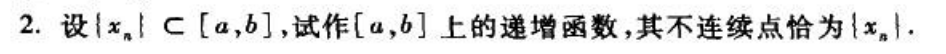
\includegraphics[width=\textwidth]{hw15-2025061016.png}
% \caption{}
\label{}
\end{figure}
\end{exercise}
\[
f(x)\coloneqq \sum_{n=1}^{\infty} \frac{1}{n^{2}}\chi_{[x_n,b]}(x)
\]
首先这个函数良好定义,对于任意给定的 $x\in[a, b]\setminus \{ x_n \}$,对于任意 $\epsilon>0$,都存在 $\delta=\min_{n\geq1}\lvert x-x_n \rvert>0$,使得
\[
\lvert f(x)-f(y) \rvert =0\leq \epsilon \qquad \forall y\in(x-\delta,x+\delta)\cap[a,b]
\]
而对于任意给定的 $x_n$,对于任意 $\delta>0$,$f$ 在 $x_n$ 处跳跃,故
\[
\left\lvert  f\left( y \right)-f(x)  \right\rvert=\frac{1}{n^{2}}>0\qquad \forall y\in(x-\delta,x)\cap[a,b]
\]
\begin{exercise}
\begin{figure}[H]
\centering
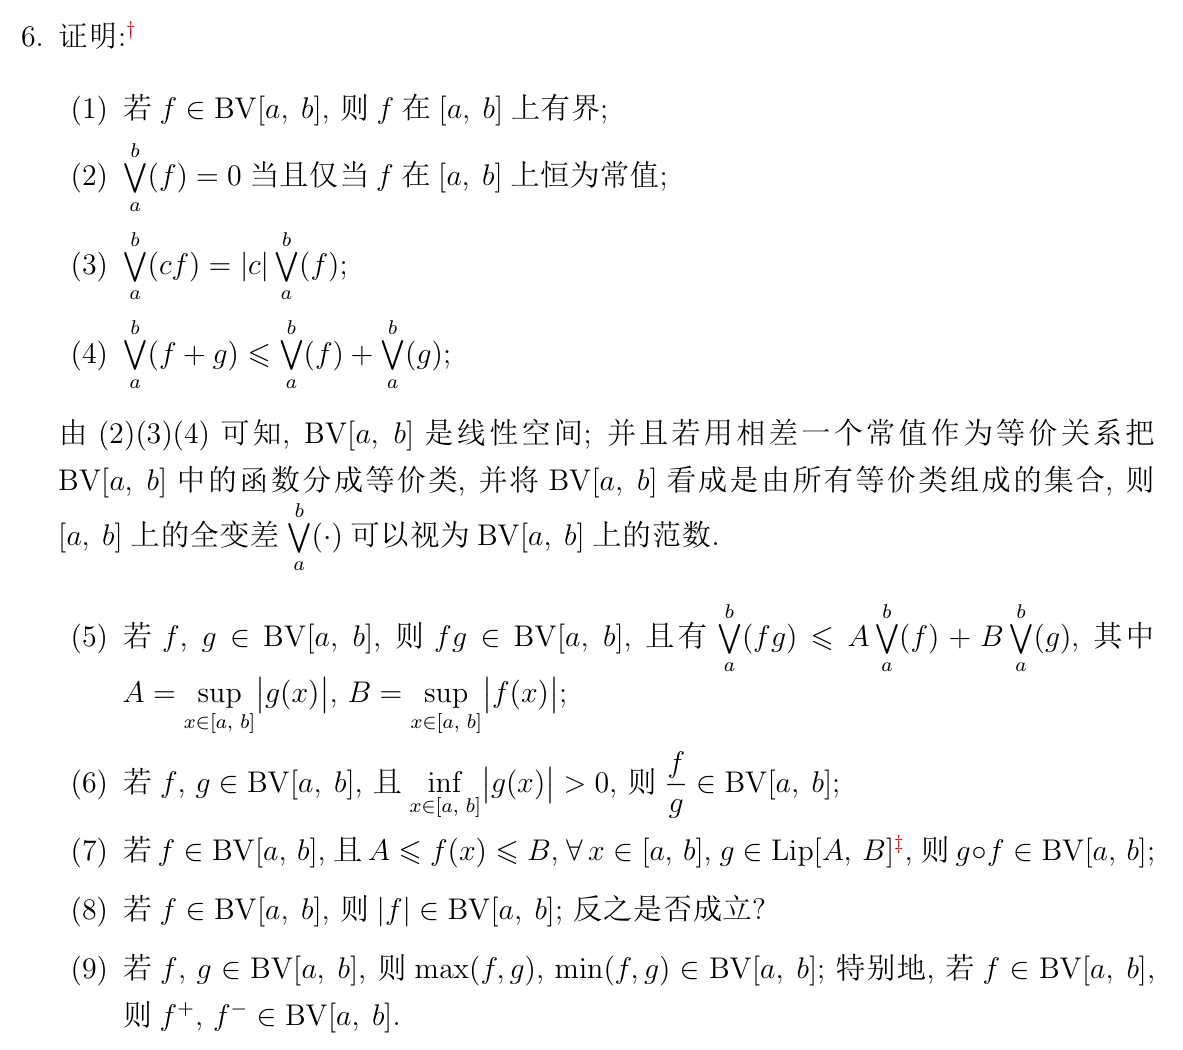
\includegraphics[width=\textwidth]{1-hw15-2025061016.png}
% \caption{}
\label{}
\end{figure}
\end{exercise}
\begin{figure}[H]
\centering
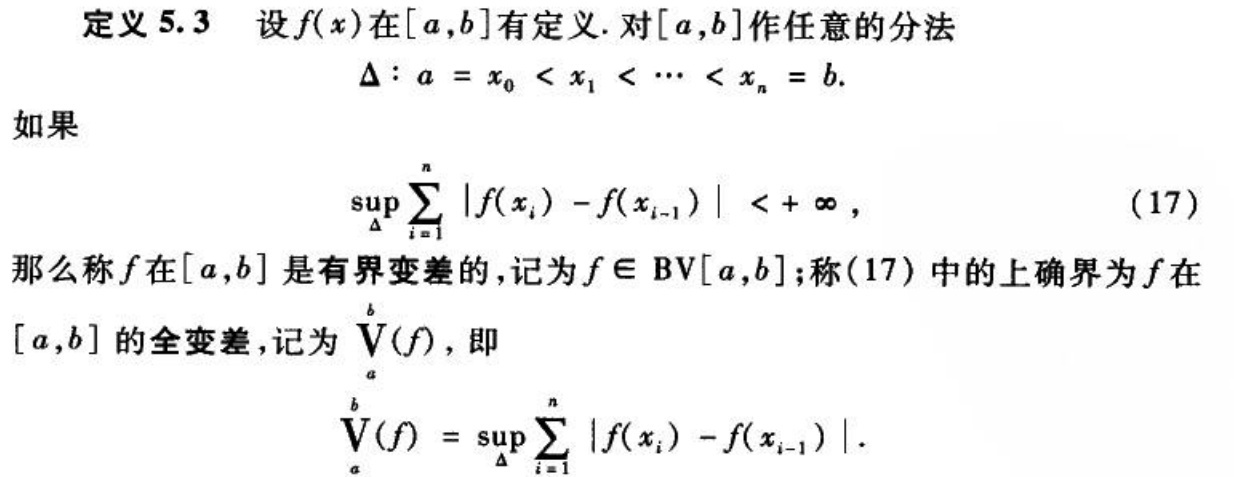
\includegraphics[width=\textwidth]{2-hw15-2025061016.png}
% \caption{}
\label{}
\end{figure}

\begin{figure}[H]
\centering
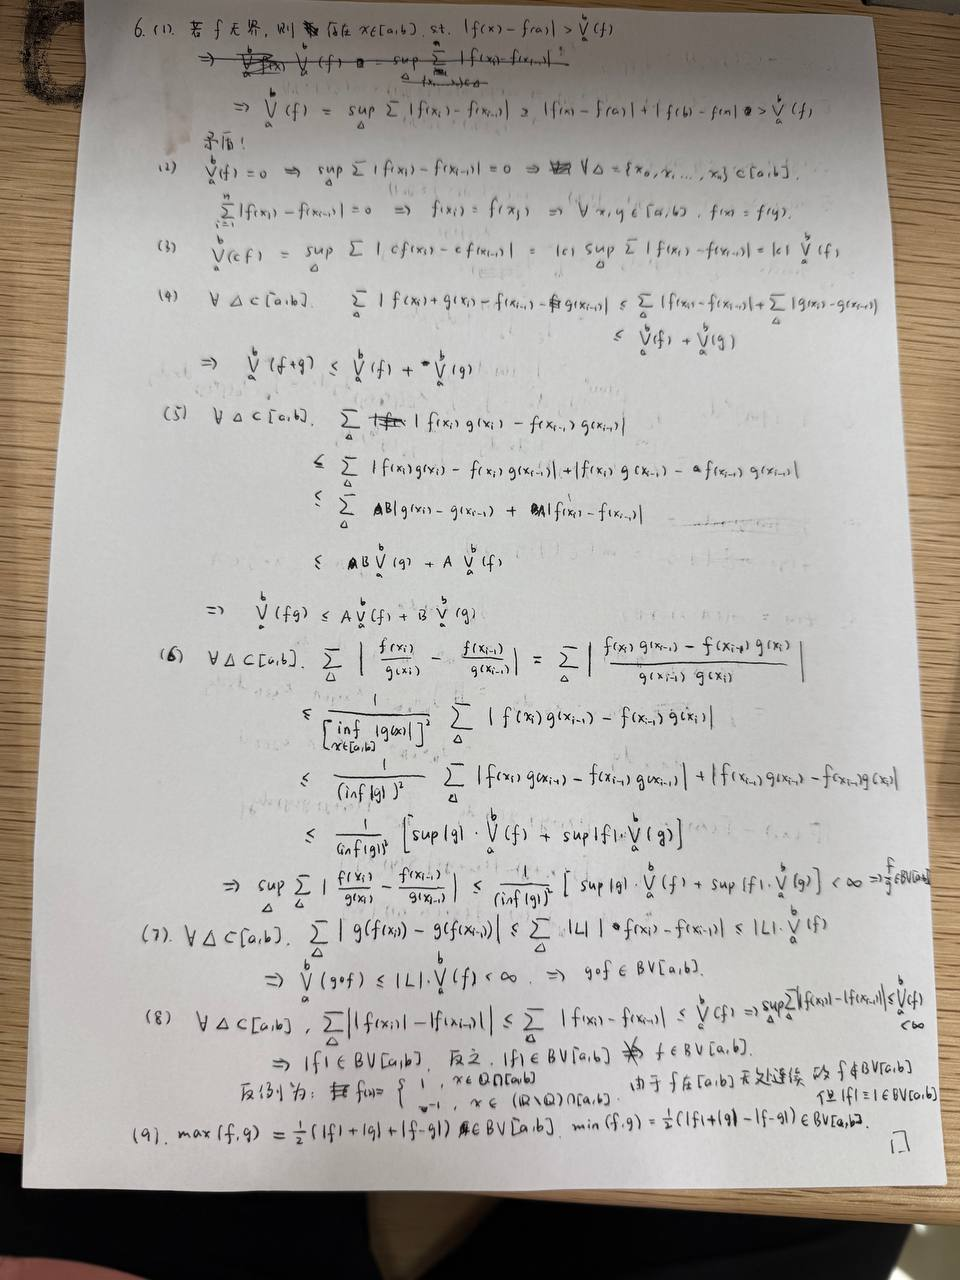
\includegraphics[width=\textwidth]{1-hw15-2025061017.png}
% \caption{}
\label{}
\end{figure}

\begin{exercise}
\begin{figure}[H]
\centering
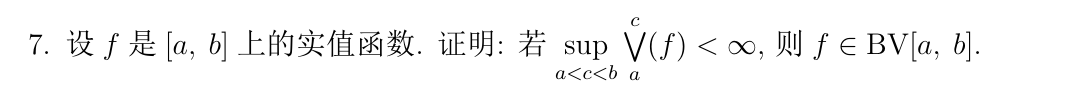
\includegraphics[width=\textwidth]{hw15-2025061017.png}
% \caption{}
\label{}
\end{figure}
\end{exercise}
\begin{figure}[H]
\centering
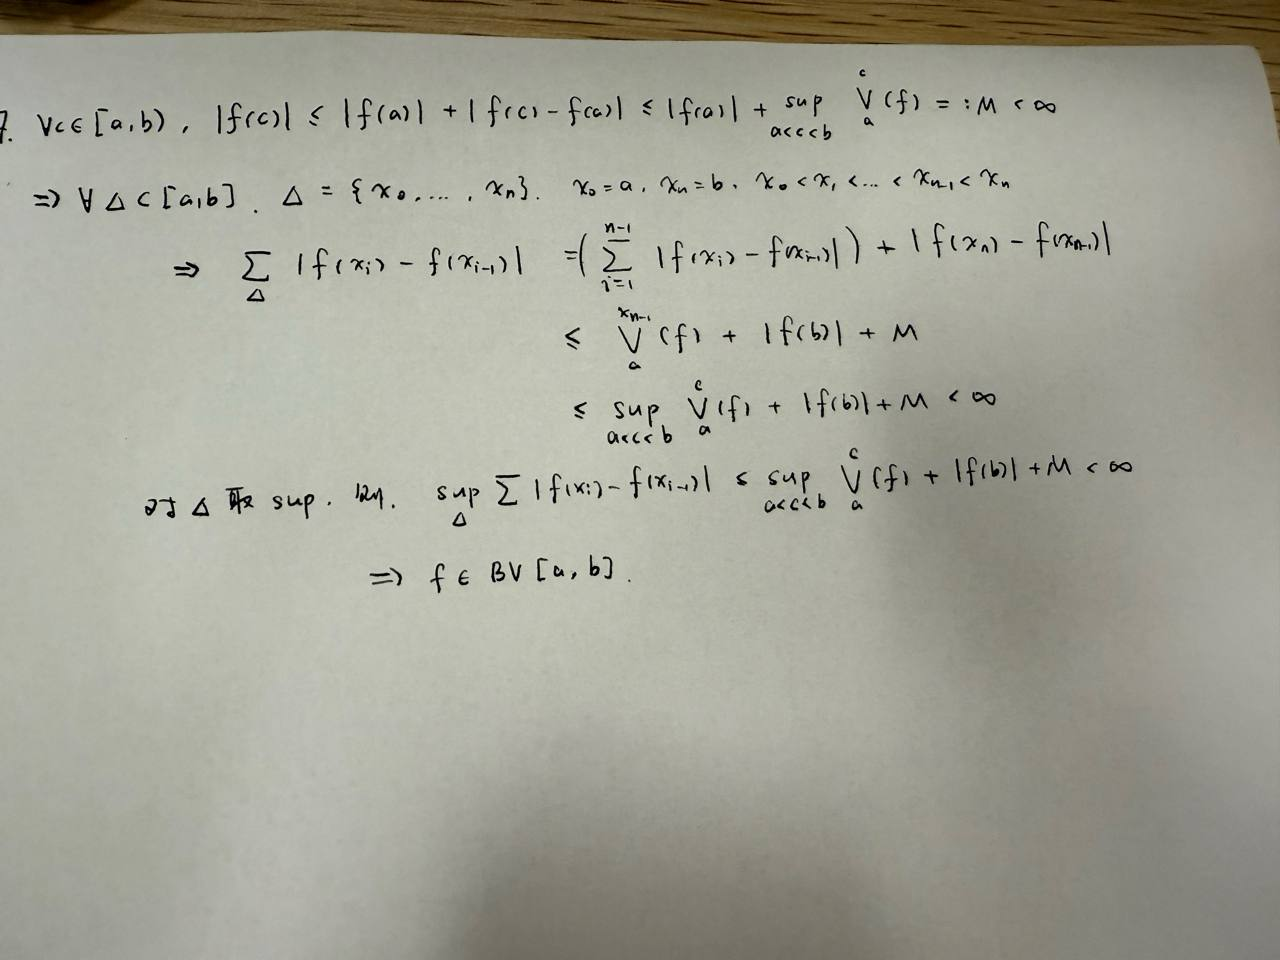
\includegraphics[width=\textwidth]{3-hw15-2025061017.png}
% \caption{}
\label{}
\end{figure}

\begin{exercise}
\begin{figure}[H]
\centering
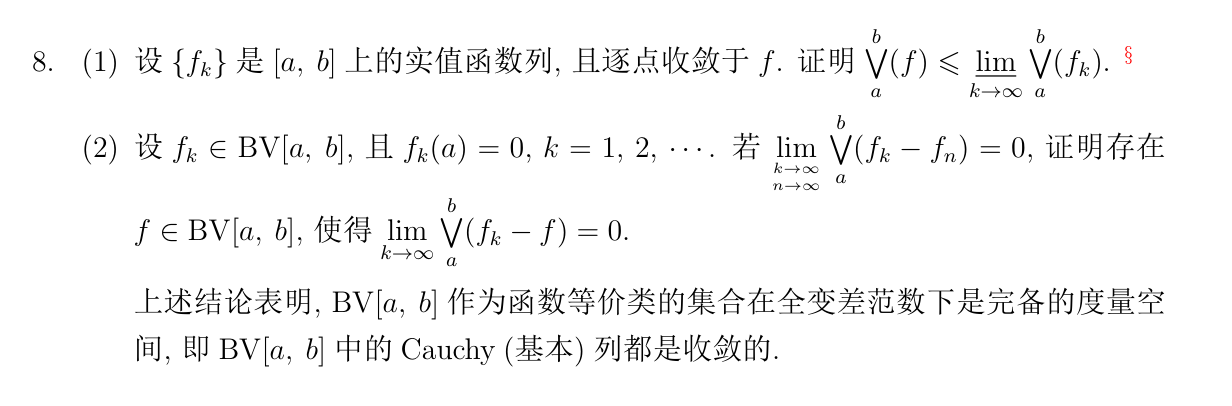
\includegraphics[width=\textwidth]{2-hw15-2025061017.png}
% \caption{}
\label{}
\end{figure}
\end{exercise}
\begin{figure}[H]
\centering
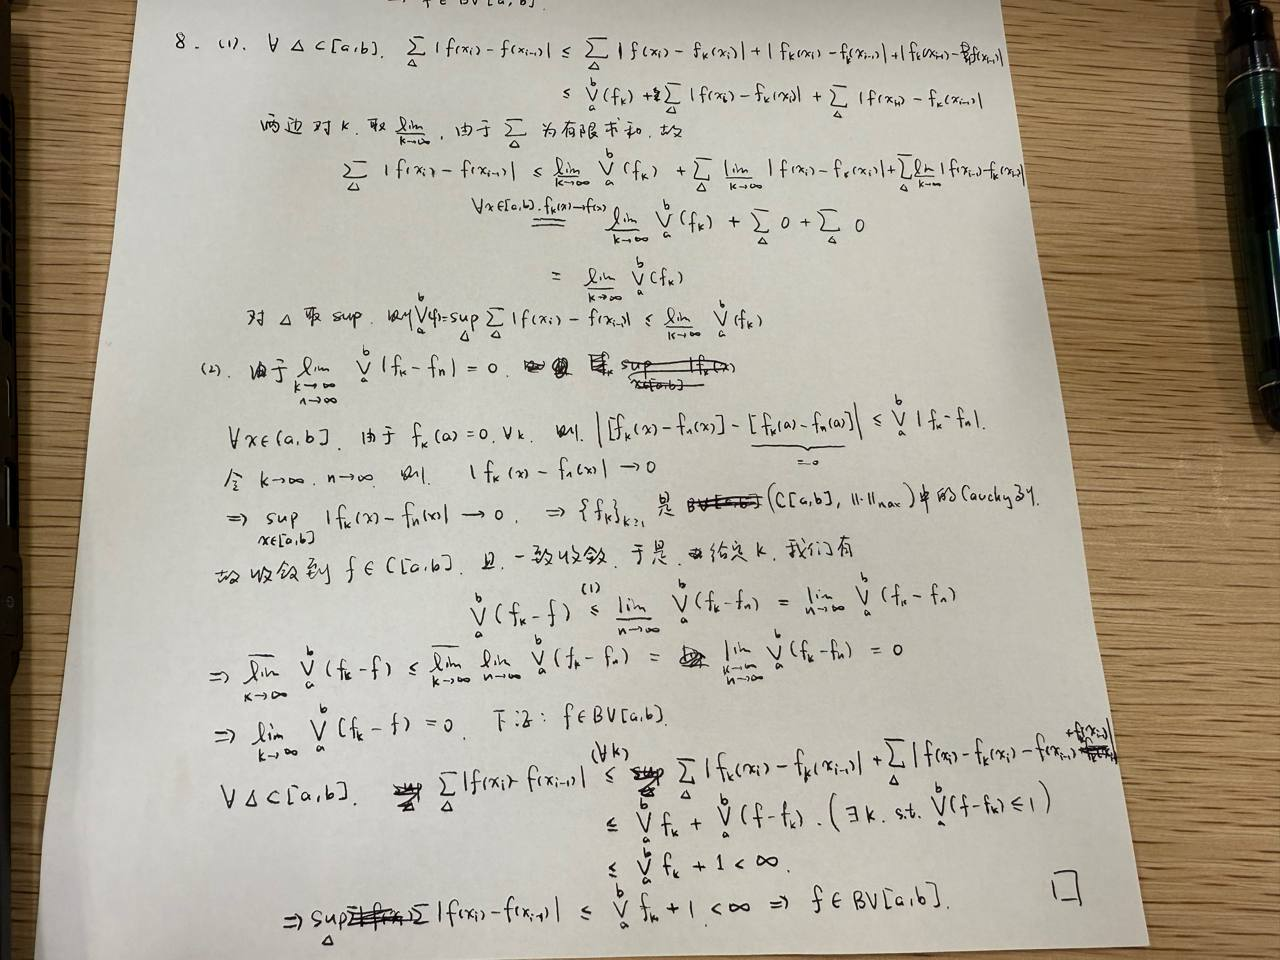
\includegraphics[width=\textwidth]{4-hw15-2025061017.png}
% \caption{}
\label{}
\end{figure}
